\section{ManageOrders-Service}

\subsection{Allgemeines}

Der Manage-Orders-Service bietet die Funktionalitäten, die benötgit werden, damit der Nutzer in der
App neue Bestellungen erzeugen und vergangene für die Zahlungsabwicklung vor Ort abfragen und
deren QR-Code vorzeigen kann.

\subsubsection{API-Routes}

\begin{code}
    \centering
    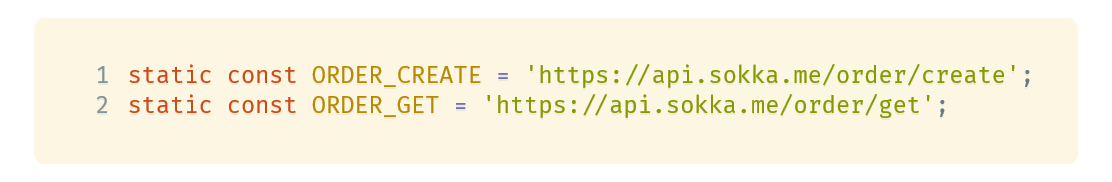
\includegraphics[width=1\textwidth]{images/Client/services/manage-orders/orderRoutes.png}
    \vspace{-25pt}
    \caption{Benötigte Routes der Sokka-API zur Verwaltung von Nutzer-Bestellungen}
\end{code}

\subsection{Generieren einer neuen Bestellung}

Sobald ein Nutzer die in seinem Warenkorb befindlichen Waren bestellt, wird ein API-Request abgesendet,
der in der Datenbank einen neuen Bestell-Eintrag erzeugt und abrufbar macht.

Hierfür müssen alle Menüs und Produkte, die der Nutzer bestellen möchte, als Payload an den
Request übergeben werden.\\
Diese werden per \lstinline{loadMenus()}- sowie \lstinline{loadProducts()}-Funktion
in den Body des Requests geschrieben.

\begin{code}
    \centering
    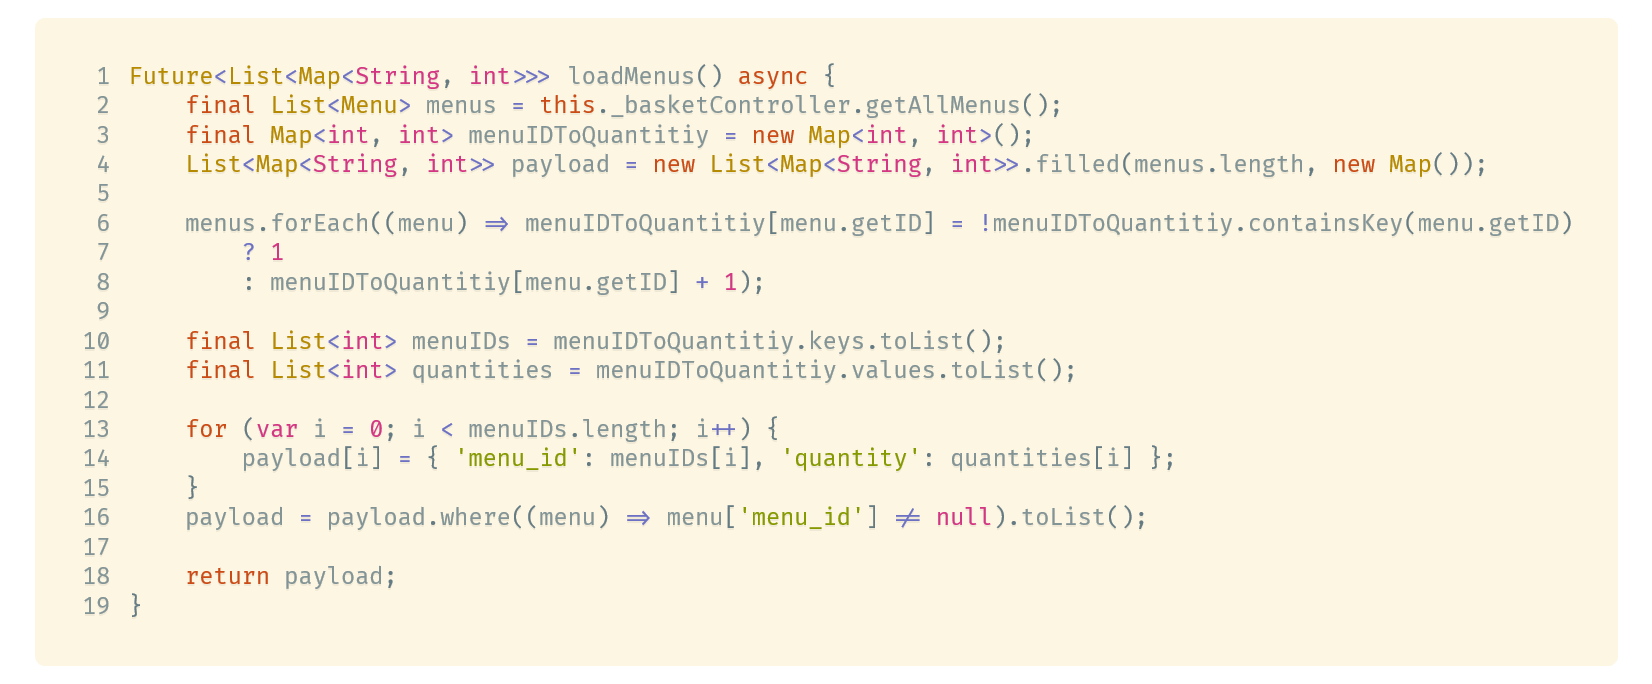
\includegraphics[width=1\textwidth]{images/Client/services/manage-orders/createMenuPayload.png}
    \vspace{-25pt}
    \caption{\lstinline{loadMenus()}-Funktion zum Laden bestellter Menüs in den Request-Body}
\end{code}

\begin{code}
    \centering
    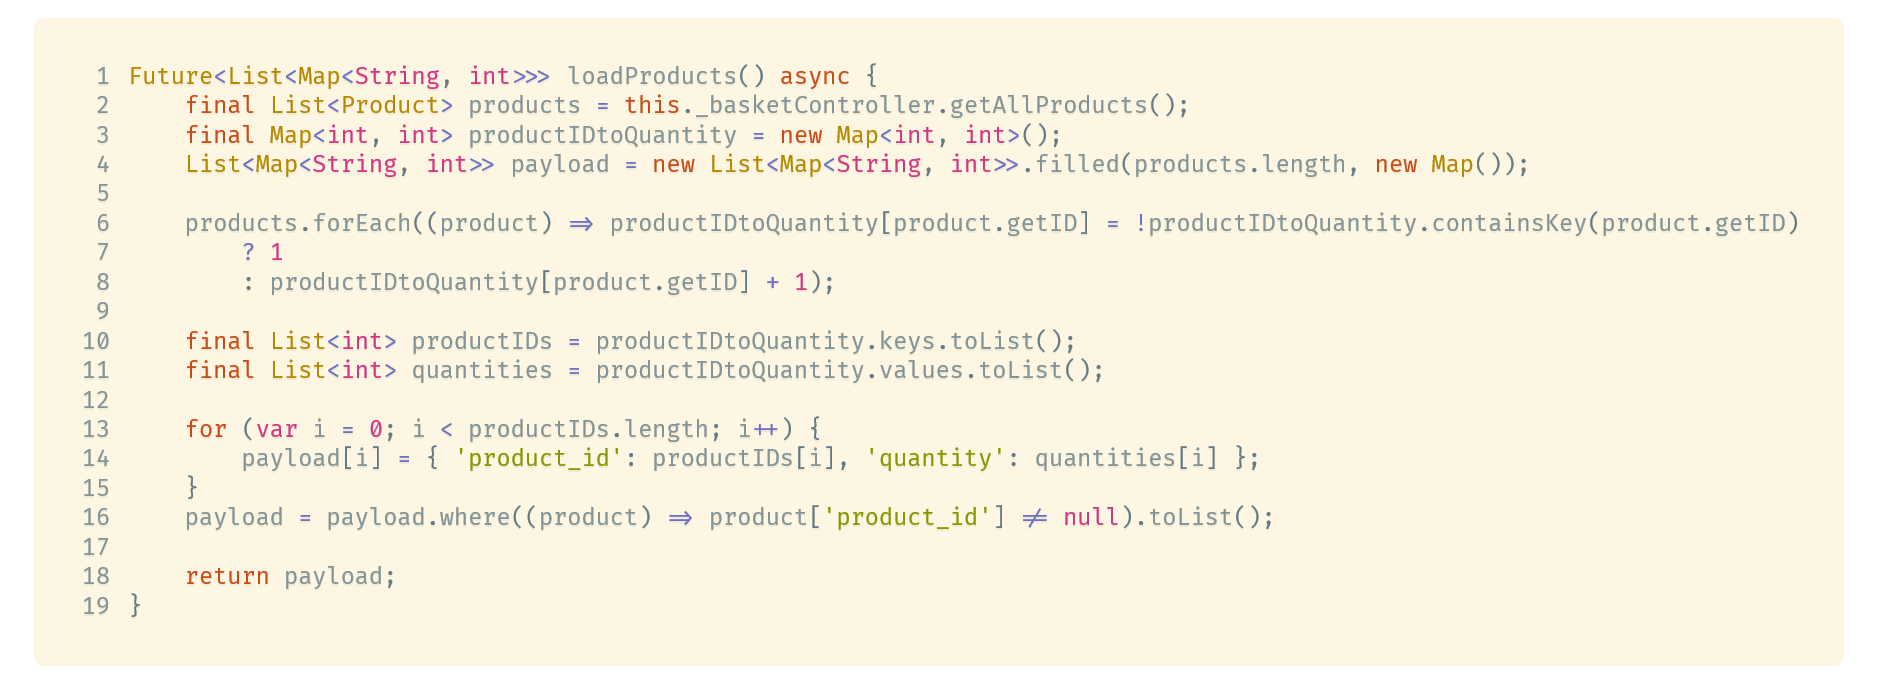
\includegraphics[width=1\textwidth]{images/Client/services/manage-orders/createProductPayload.png}
    \vspace{-25pt}
    \caption{\lstinline{loadProducts()}-Funktion zum Laden bestellter Produkte in den Request-Body}
\end{code}

\newpage

Jene Funktionen können nun in der \lstinline{createOrder()}-Funktion aufgerufen werden.

\begin{code}
    \centering
    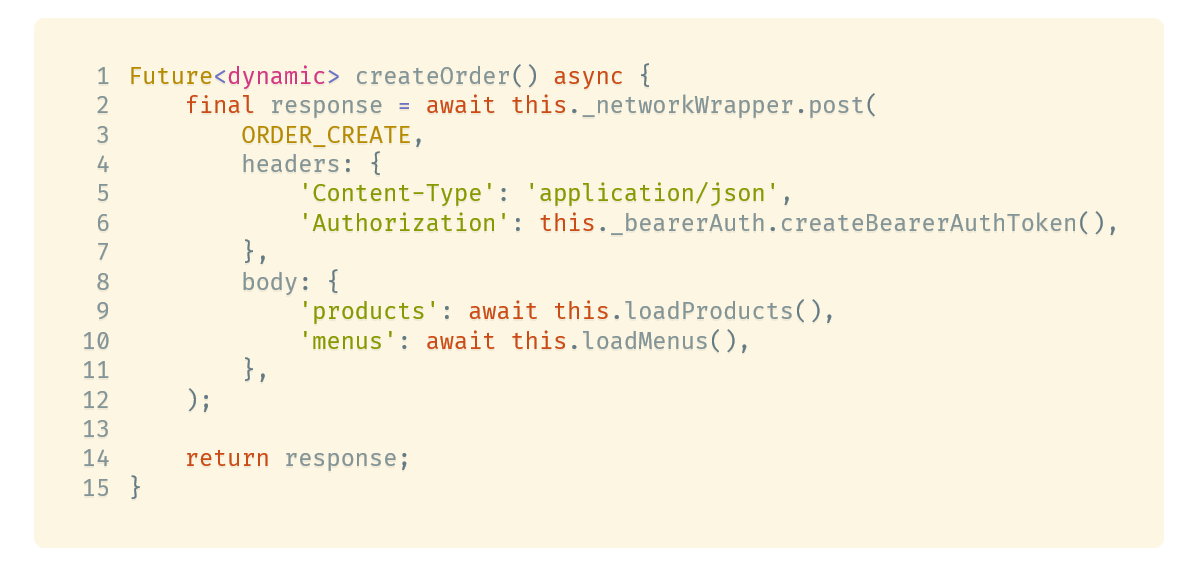
\includegraphics[width=1\textwidth]{images/Client/services/manage-orders/createOrder.png}
    \vspace{-25pt}
    \caption{\lstinline{loadProducts()}-Funktion zum Laden bestellter Produkte in den Request-Body}
\end{code}

Ist der Request erfolgreich, wird eine neue Bestellung in der Datenbank erzeugt und im 
\lstinline{Order-View} dargestellt, damit der QR-Code der eben aufgegebenen Bestellung
direkt zum Abruf bereit steht.

\newpage

\subsection{Abfragen der Bestellungen eines Nutzers}

Damit ein Nutzer Einblick über seine vergangenen Bestellungen hat und diese aufrufen zum Scan 
bei der Zahlungsabwicklung vorzeigen kann, werden alle getätigten Bestellungen des Nutzers bei App-Start
der Liste des \lstinline{Order-Controllers} übergeben, um im \lstinline{Order-View} angezeigt werden zu können.

Dies geschieht mithilfe der \lstinline{appendOrders()}-Funktion des Services.

\begin{code}
    \centering
    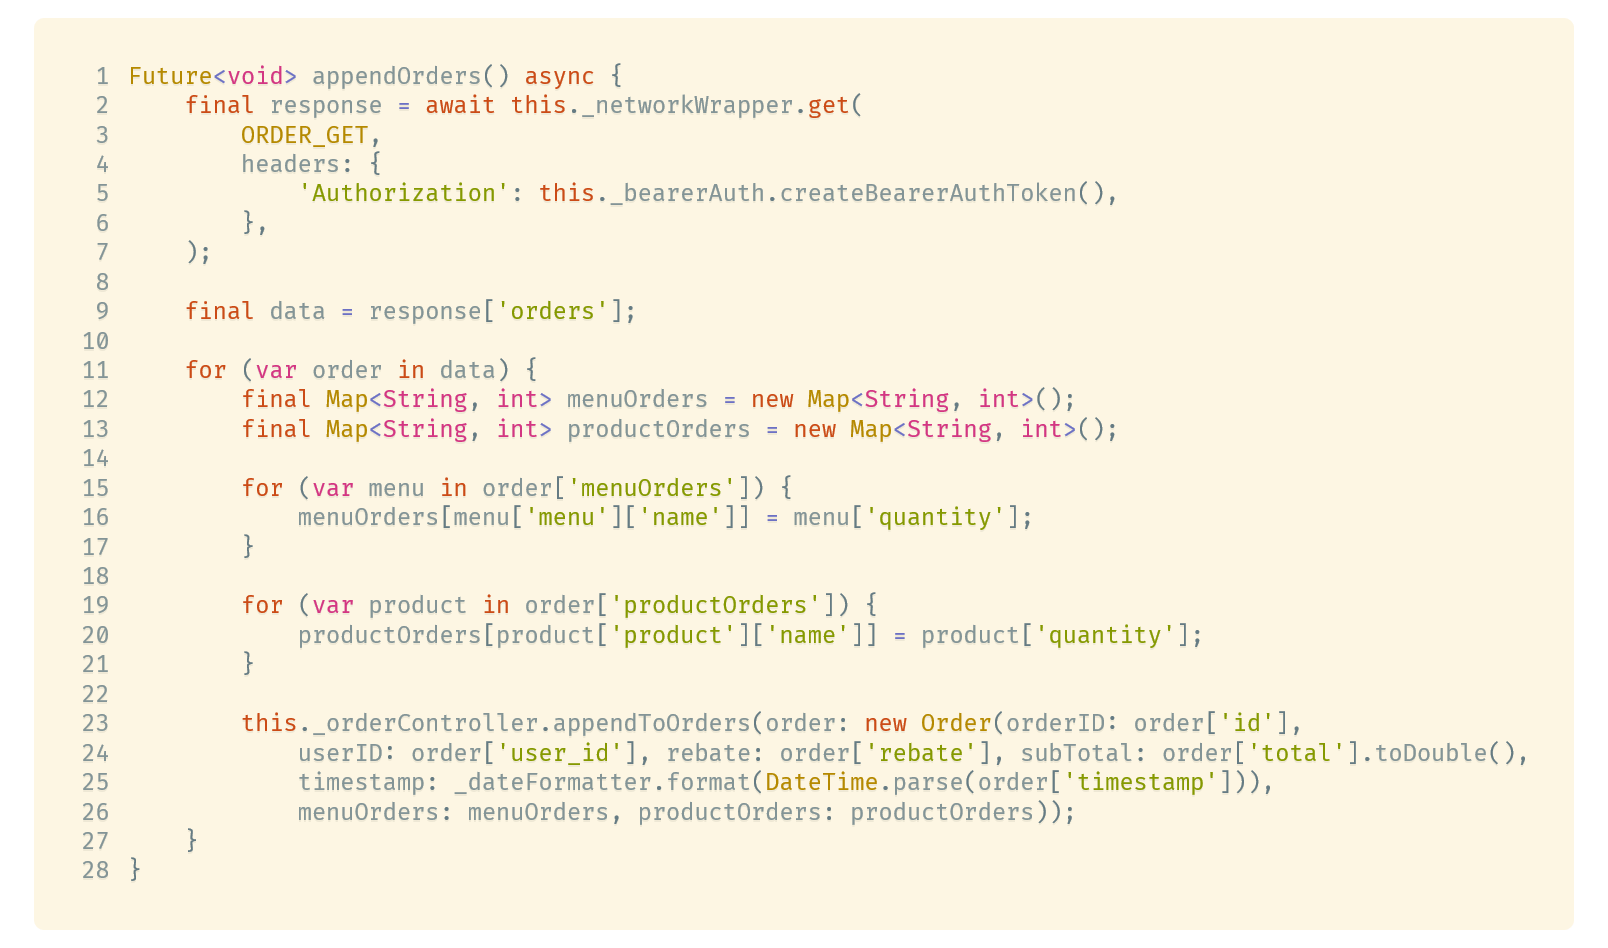
\includegraphics[width=1\textwidth]{images/Client/services/manage-orders/appendOrders.png}
    \vspace{-25pt}
    \caption{Funktion zum Abfragen aller vom Nutzer getätigten Bestellungen}
\end{code}